% !TeX root = ../main.tex
% Add the above to each chapter to make compiling the PDF easier in some editors.

\chapter{Implementation}\label{chapter:implementation}
Chapter Introduction


\section{Concept: Features and Interaction Capabilities of the App}
In this section, we explore the expected features and capabilities crucial for our objectives and the necessary interaction capabilities from an end user's perspective.\\
We start with the visualisation capabilities of the benchmark data, where the goal is to easily identify performance bottlenecks. This involves pinpointing interesting queries with distinct performances for subsequent in-depth analysis.\\
For deeper analysing and achieving a profound understanding of diverse performance results within queries, the application should support a focus on individual queries. Users should be able to view the performance of a single query from various perspectives, providing a comprehensive image. Comparative analysis across queries from different database systems or even the same database but with different configurations is also essential.\\ 
Then, we examine the requirements for a suitable dashboard that contains the main part of the performance visualisations. Multiple views are necessary to construct a complete understanding of the current point of interest. The optimal structure of these views may vary depending on the point of interest. The flexibility of a drag-and-drop solution for structuring views allows users to tailor the overview according to their specific interests.\\
Finally, we examine the capability of the system to facilitate collaboration and knowledge sharing. The application should enable the saving and sharing of potential findings. This involves saving the interface configuration of the analysis for sharing with other users. Recipients should be able to upload the received configuration, gaining access to the same data and visualisation structure for collaborative exploration.


\subsection{Visualising Benchmark Data}
Visualising Benchmark Data includes multiple aspects. It involves the import of the actual data, where a proper way of importing the data should be provided. We also cover the utilized plots and charts for the data visualisation. In addition to visualisation, we offer a comprehensive table view of the data.


\subsubsection{Charts and Plots}

We aim to offer a dashboard containing multiple data views. To prevent UI clutter, a universal legend of database system instances is suitable, eliminating the necessity to display a legend in every chart. In the legend depicted in Figure~\ref{fig:legend} all database systems included in the benchmark data are presented as coloured toggles, allowing users to activate or deactivate their appearance in the visualisation.

\begin{figure}[h]
    \centering
    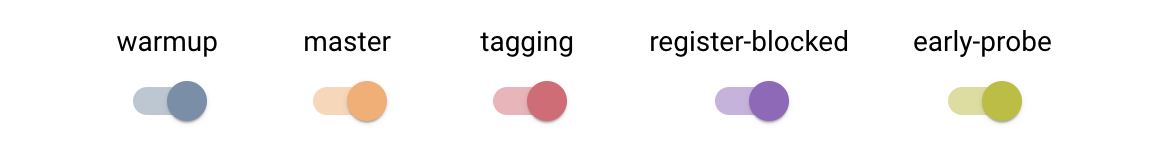
\includegraphics[width=1\linewidth]{figures/legend.png}
    \caption{Gobal legend of all database systems contained in the imported performance data.}
    \label{fig:legend}
  \end{figure}



When initiating the analytical process with the Benchy Viewer after importing the benchmark data, it may be beneficial to start with a general and straightforward overview of the benchmark data for quickly gaining an understanding of the general performance standings of the database systems.\\
Within the Benchy Viewer, this overview is effectively conveyed through the relative performance visualisation, as depicted in Figure~\ref{fig:relative-performance}. This chart displays, on the Y-Axis, the relative performance of each system in percentage compared to the best-performing system in the benchmark data. The X-Axis lists and represents every database system contained in the benchmark data.

\begin{figure}[h]
  \centering
  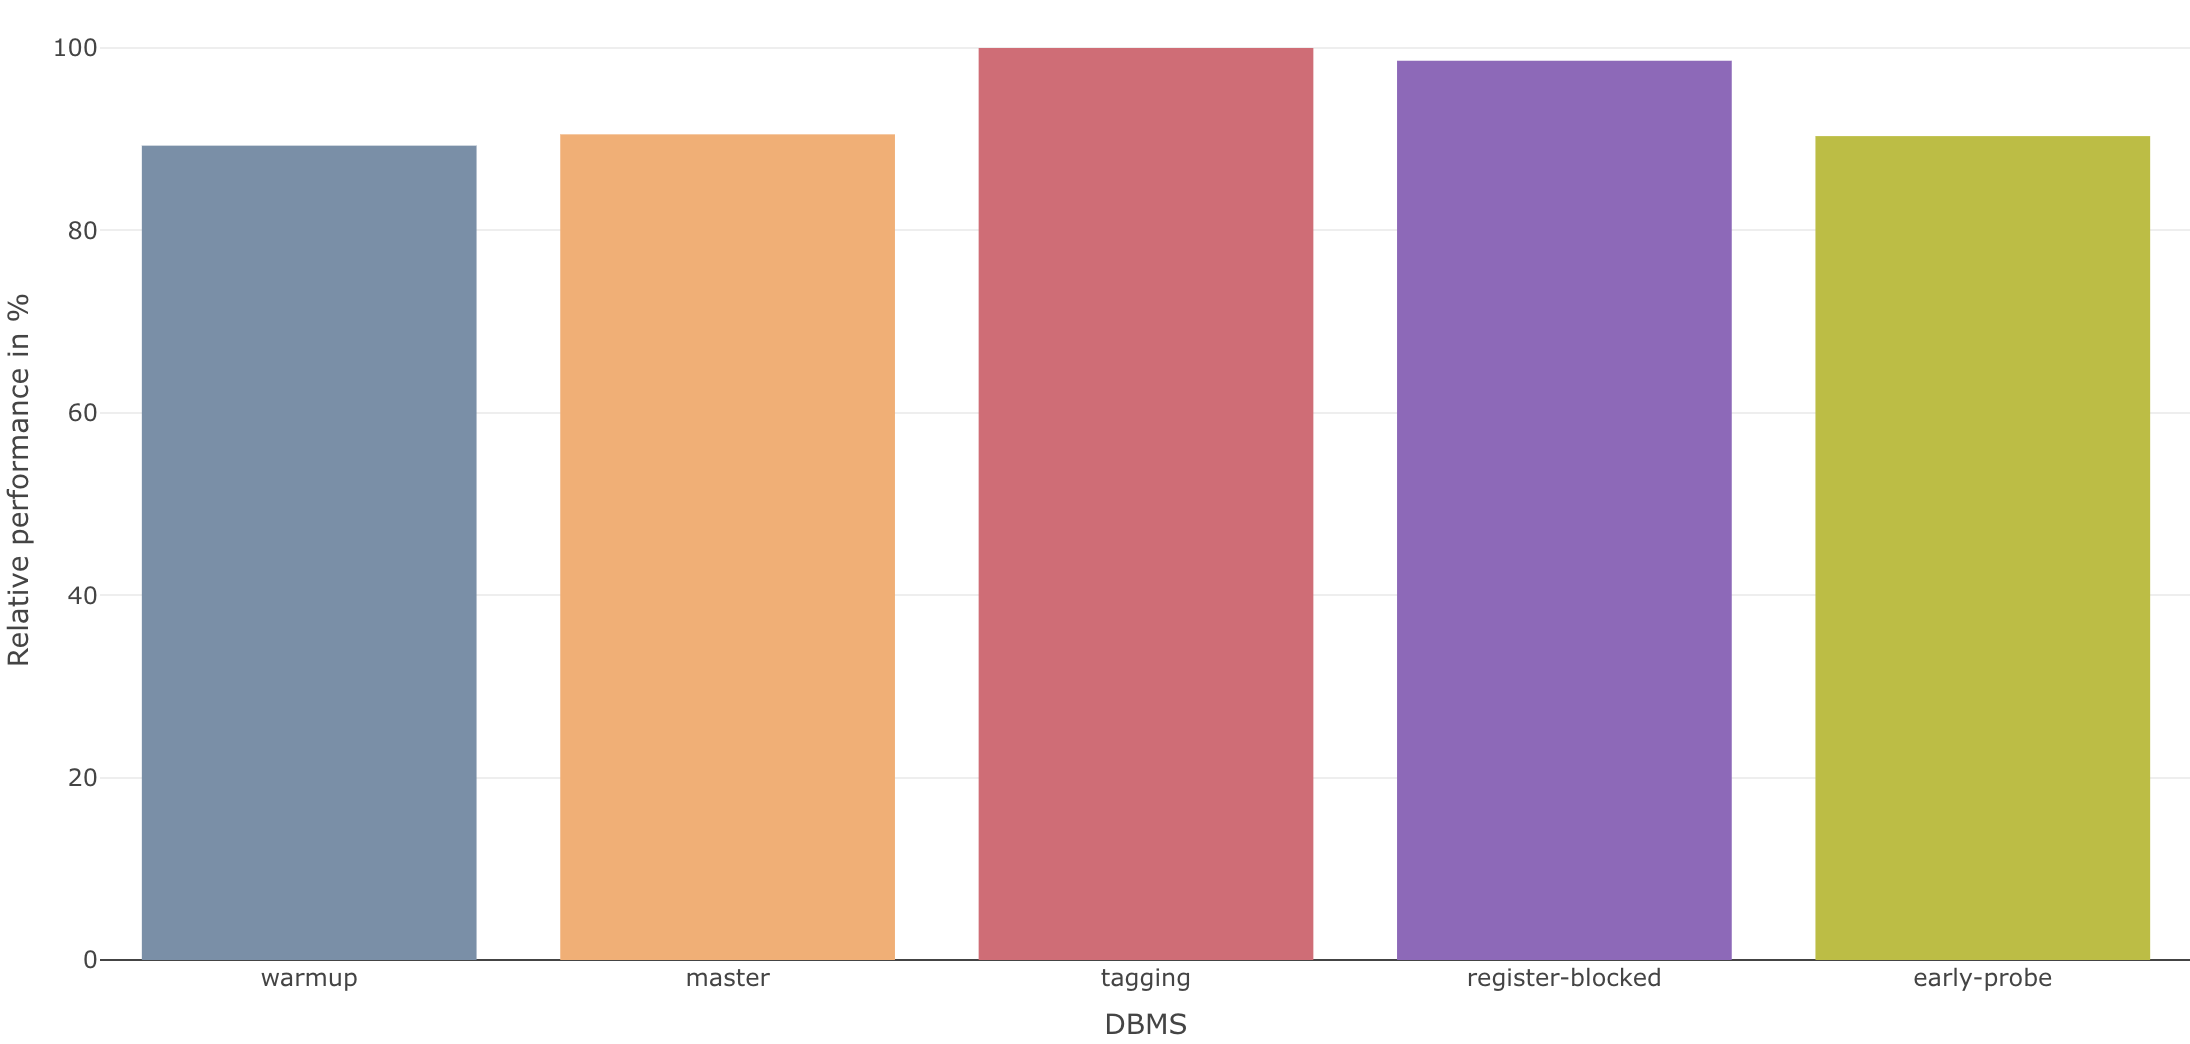
\includegraphics[width=1\linewidth]{figures/bsp-relative-performance.png}
  \caption{Bar chart visualises the relative performance of all systems compared to the best performing system.}
  \label{fig:relative-performance}
\end{figure}

After obtaining this initial overview, users can quickly identify the system marked with the red colour as the benchmark, as it processes all queries faster than all other systems. In this visualisation, this system is set as the benchmark with 100\% performance, providing a clear reference point for relative comparisons.\\
This chart serves as a valuable starting point for further in-depth analyses and allows users to grasp the overall performance landscape before delving into specific metrics or queries.

In the next phase of the analysis process, we delve into two crucial aspects: compilation and execution. Compilation is the phase where source code is translated into machine code, preparing it for execution Compilation. It is a crucial step that impacts the overall performance of the system. On the other hand, execution is the phase where the compiled code is run on the system. This step involves the actual processing of the instructions and the generation of results. The time spent in the execution phase is a key factor in determining the system's efficiency in handling tasks.

To understand how much time each database system allocates to these processes, the Benchy Viewer offers a stacked bar chart, illustrated in Figure~\ref{fig:execution-compilation}. Here, one section of the bar signifies the time spent in the compilation step, while the other represents the time spent in the execution step.

\begin{figure}[h]
  \centering
  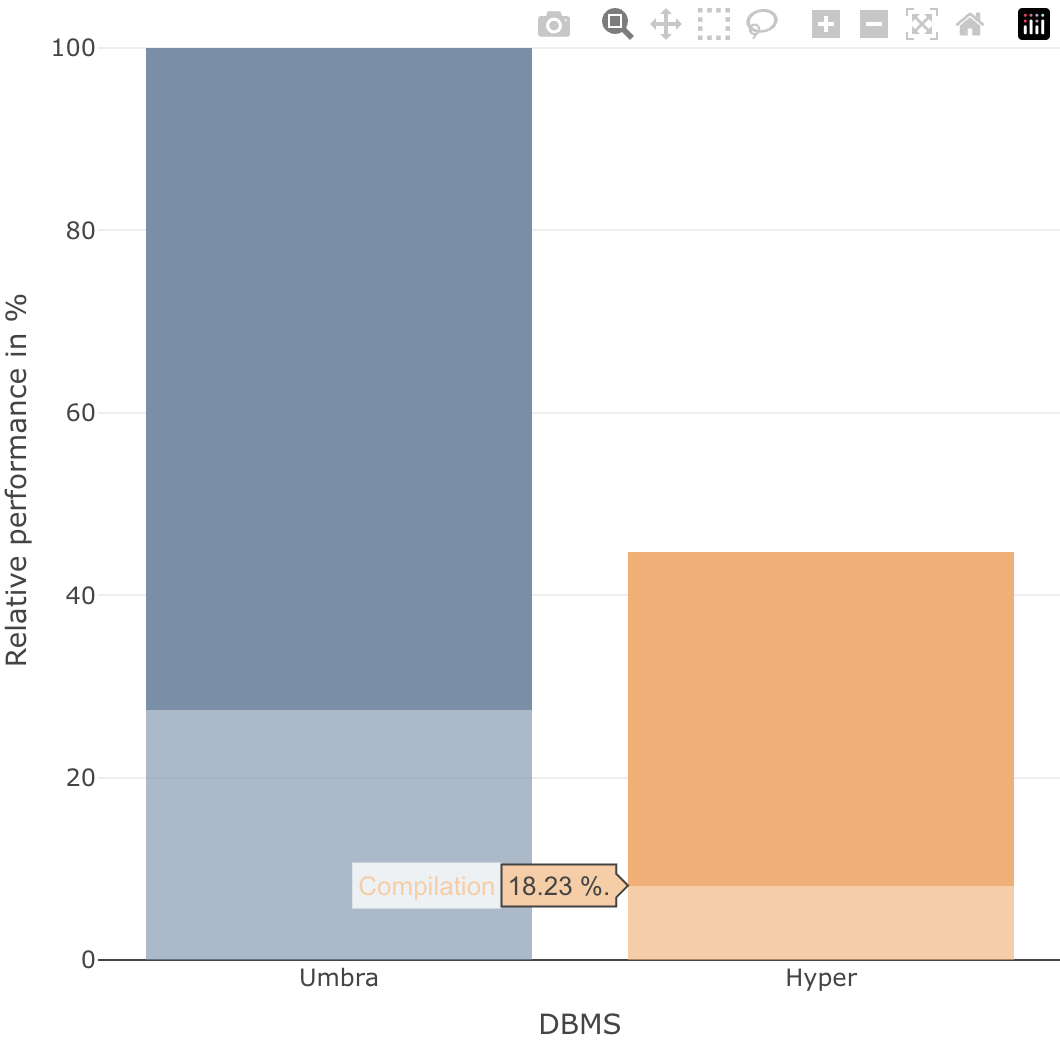
\includegraphics[width=0.5\linewidth]{figures/bsp-compilation-execution.png}
  \caption{Stacked bar chart illustrating the distribution of time between compilation and execution steps. The compilation step is depicted in a transparent accent colour, while the execution step is represented in the full colour intensity.}
  \label{fig:execution-compilation}
\end{figure}

Using solely the ratio of the two different steps, without taking into account the overall performance, would present an incomplete picture of the balance between the two process steps compared to the better-performing systems. Therefore, this chart complements the relative performance visualization discussed earlier. By incorporating information about the overall performance, it aims to offer a comprehensive understanding while illustrating the equilibrium between compilation and execution for each system.

In this example, a comparison is made between two database systems, with the Y-Axis indicating the relative performance and the X-Axis listing different database systems. Umbra stands out as the best-performing system, with its bar reaching the 100\% level. In contrast, Hyper attains 45\% of Umbra's performance. When hovering over one of the process steps, the chart displays the percentage of the total time spent by the system in that specific step. For instance, Hyper allocated 18.23\% of the entire process to the compilation step, while Umbra spent 27\% on this phase.

Hence, the stacked bar chart in the Benchy Viewer offers a consolidated view of how each database system allocates time between compilation and execution steps. Its integration of the relative performance metric ensures a balanced understanding of system efficiency, preventing oversights from focusing solely on step ratios. With clear visual distinctions and the ability to compare multiple systems, this chart enhances analytical insights into performance disparities and offering an aerial view of compilation and execution.

The preceding visualisation solution \textcolor{red}{Referenz auf PDF} shows essential benchmark visualisations, offering both a comprehensive overview of all queries and a detailed examination of each individual query.

It commences with a comparative analysis of each query using a bar chart. Similar to Figure~\ref{fig:bar-chart}, this chart displays queries from various database systems on the X-Axis, with the total time presented on the Y-Axis. 

\begin{figure}[h]
    \centering
    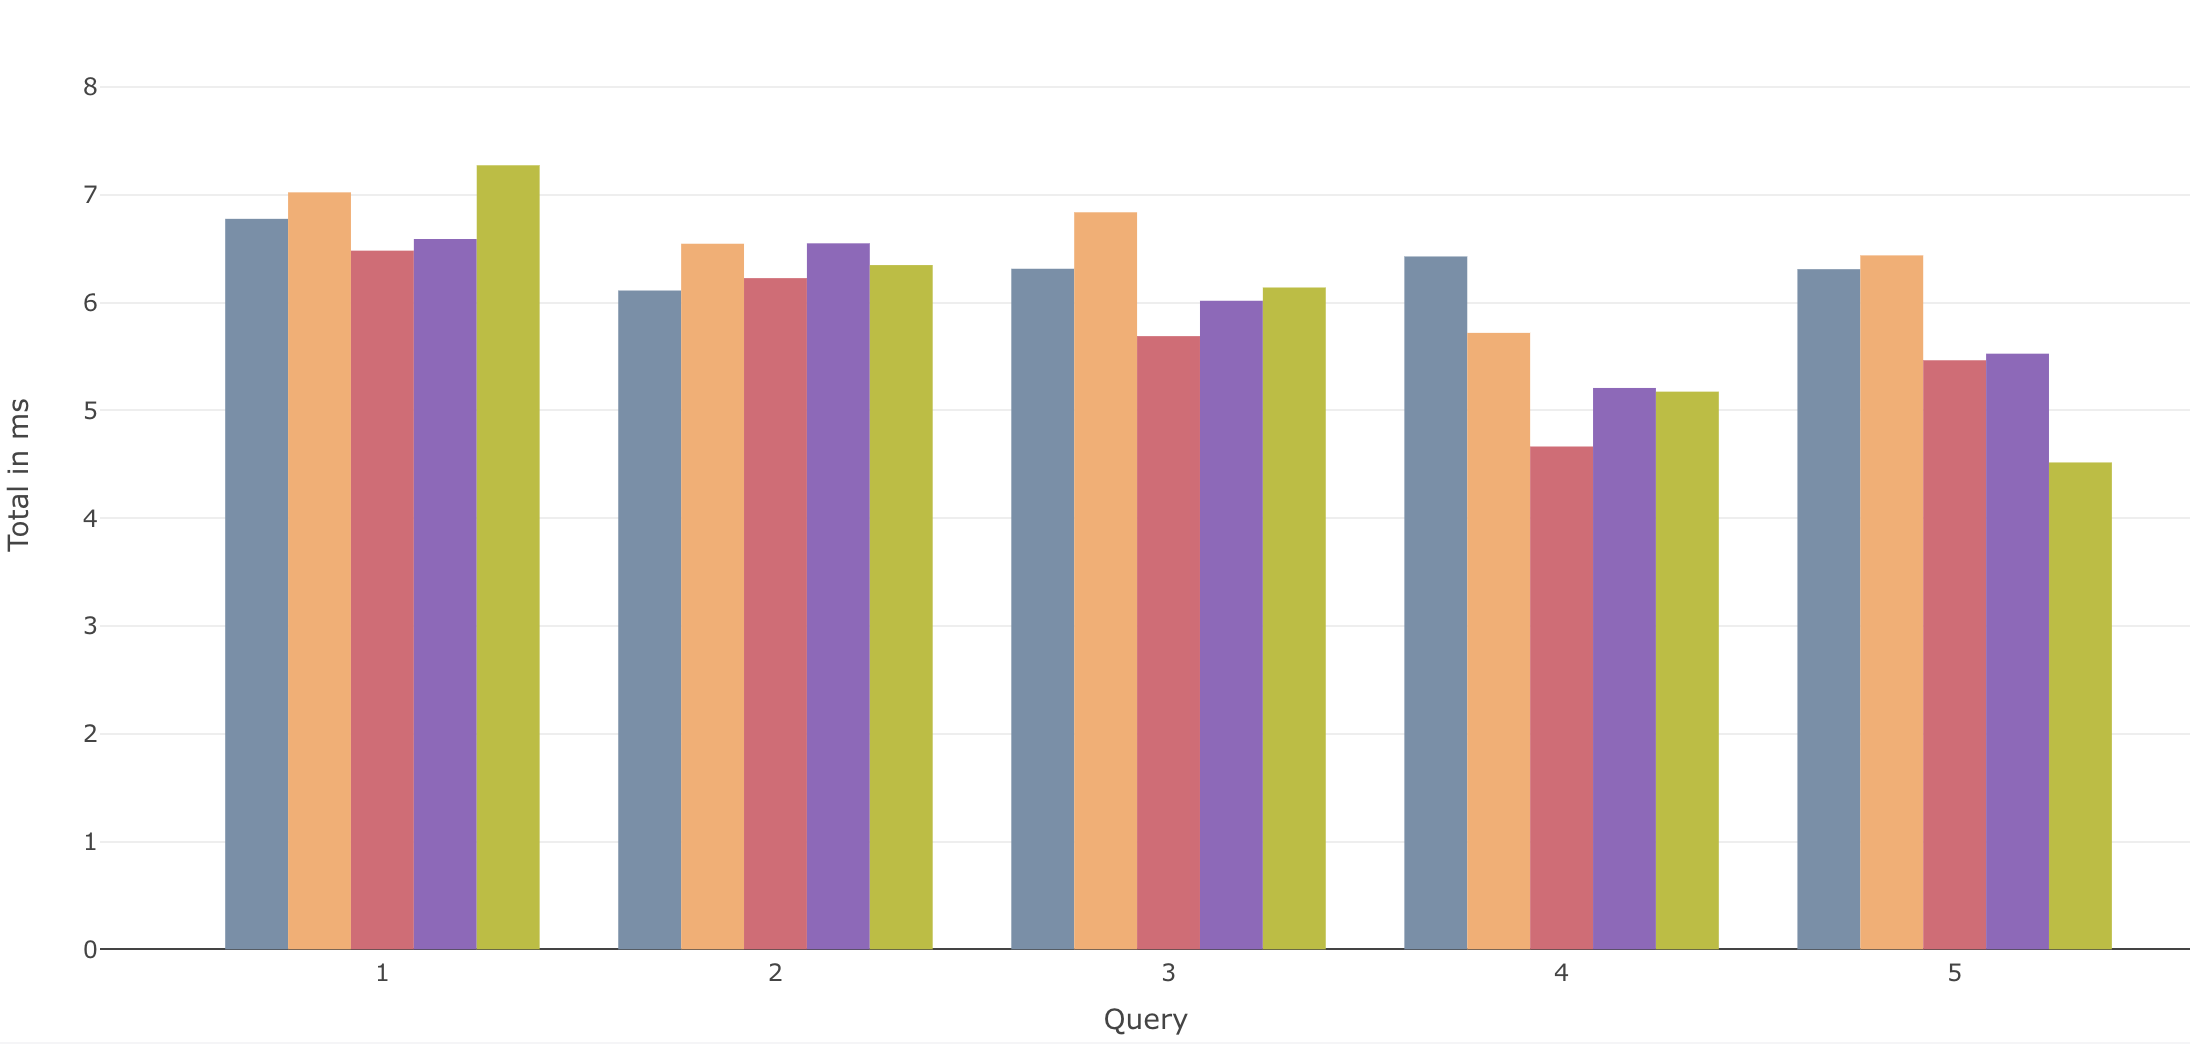
\includegraphics[width=1\linewidth]{figures/bsp-bar.png}
    \caption{Bar chart visualises the totals time in ms of different queries.}
    \label{fig:bar-chart}
  \end{figure}

Bar plots stand out as a versatile visualisation method, particularly when tasked with presenting the performance metrics of multiple queries. Their inherent clarity, with the length of each bar directly corresponding to a specific performance metric such as compilation time or execution time, makes them well-suited for diverse scenarios.\\
The straightforward visual comparison they offer is a notable strength. With each query distinctly represented by a separate bar, variations in performance become immediately apparent.\\
This quality proves especially valuable for our objective of identifying outliers, as these exceptional values are easily noticeable.

To facilitate a quick and clear overview of all queries, violin charts are employed. These charts not only provide an initial glimpse of the overall system performance but also offer distribution insights, including the shape and density of the data. They can also be combined with box plots to get a concise summary of the distribution of the results, displaying key statistics such as the median and quartiles.

\begin{figure}[h]
    \centering
    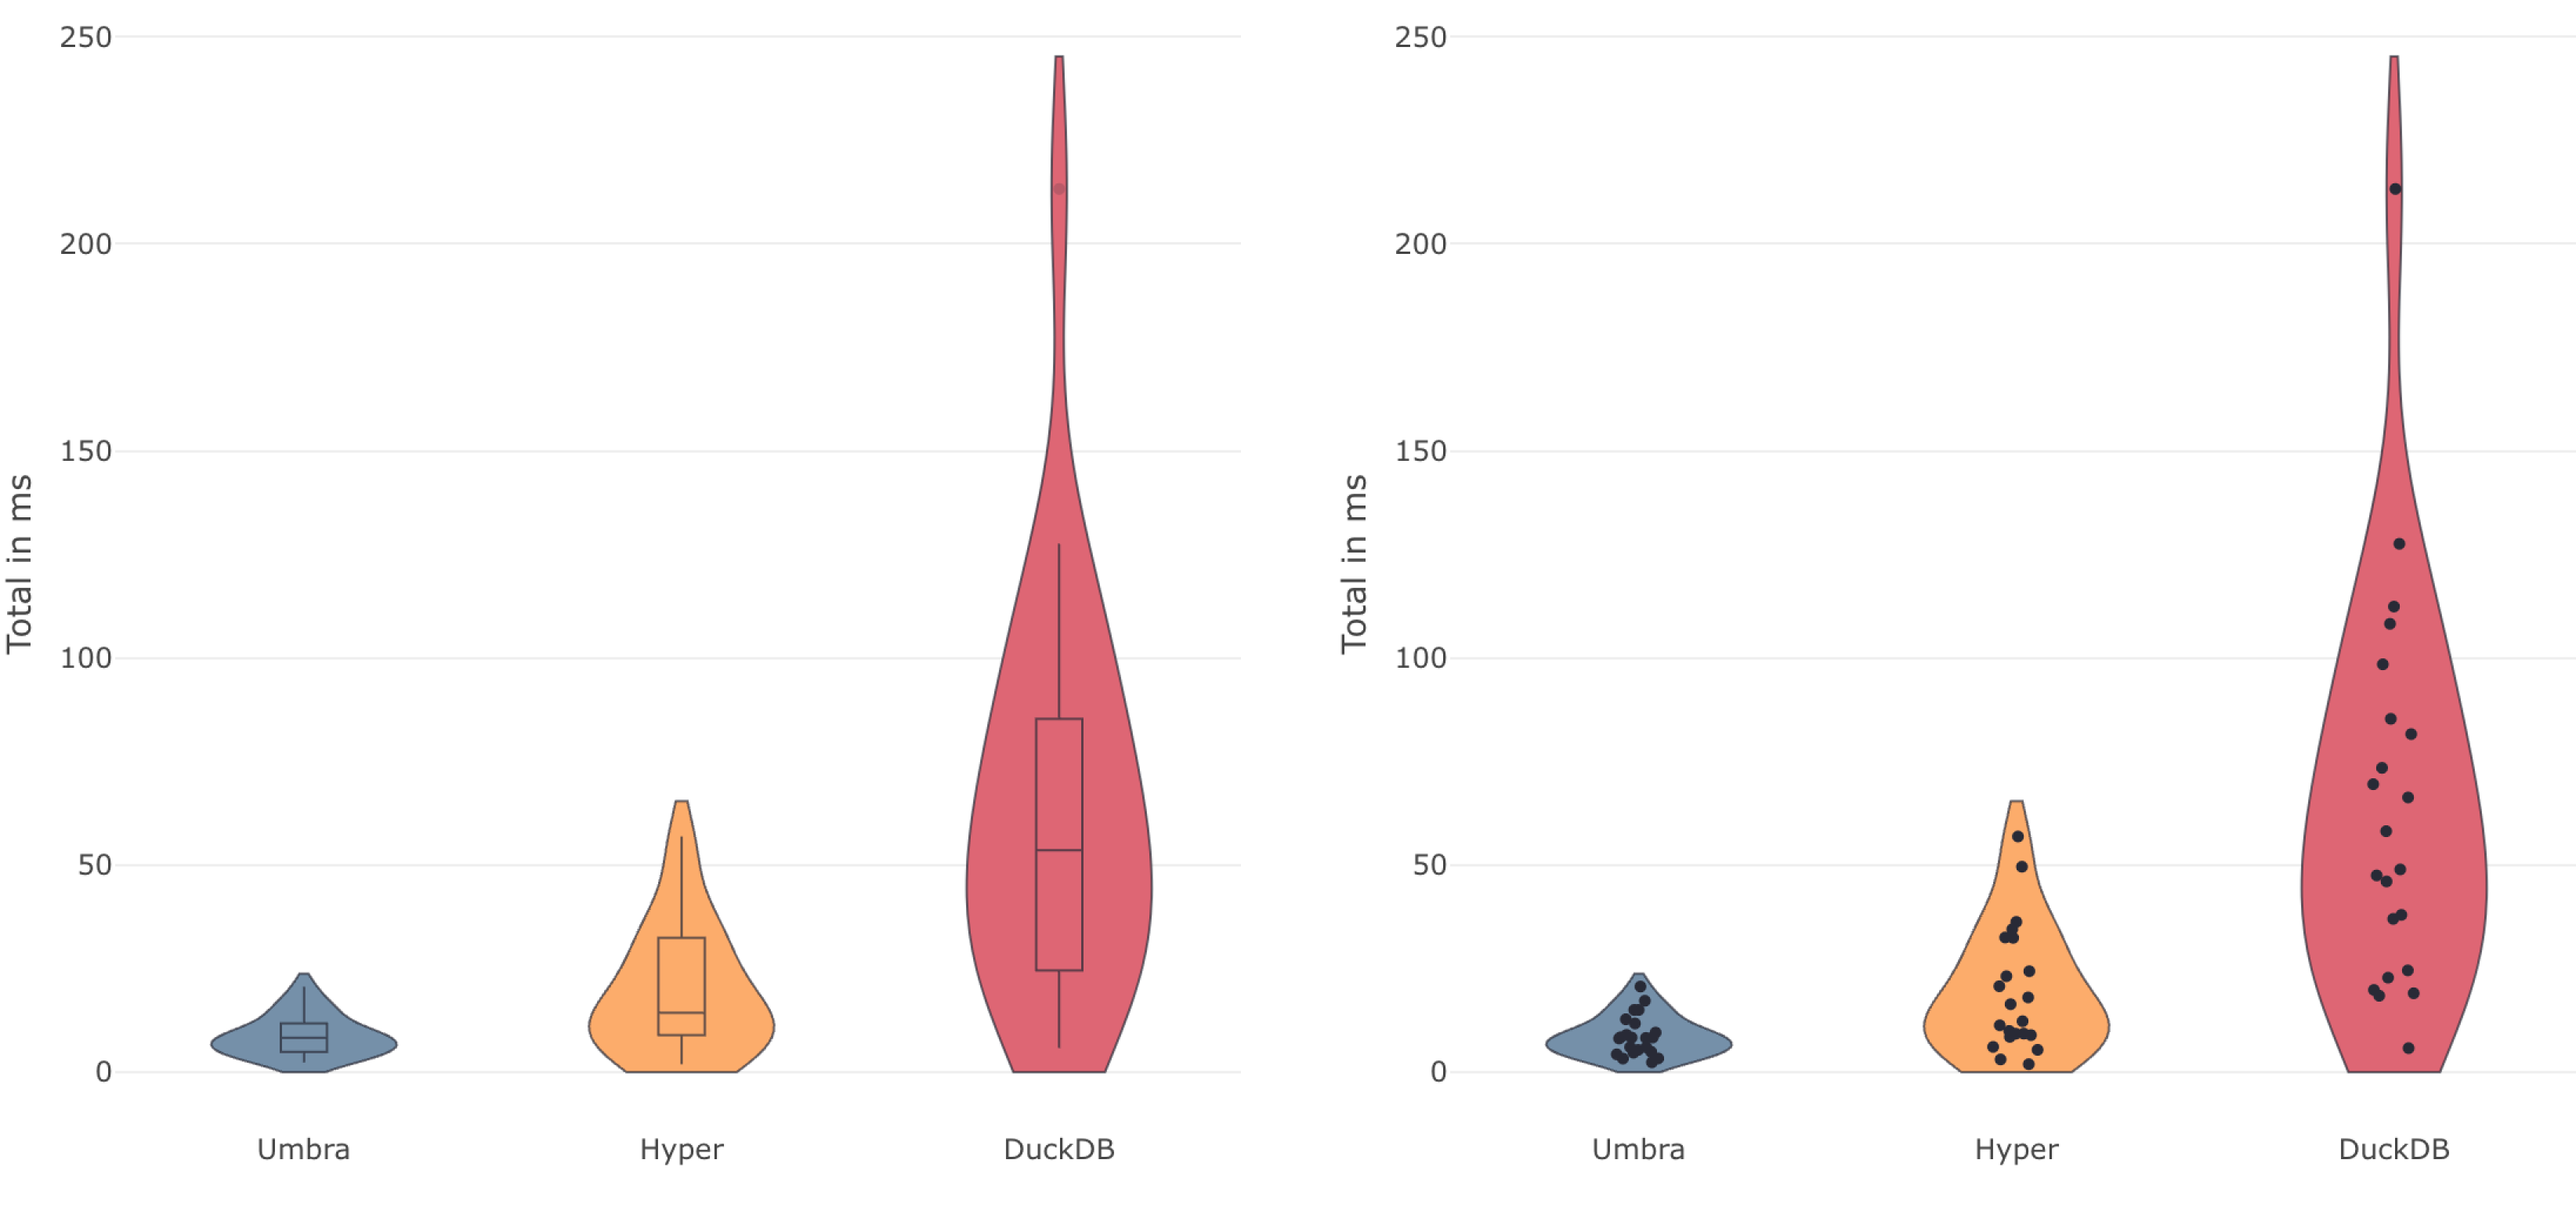
\includegraphics[width=1\linewidth]{figures/bsp-violin-boxplot-points.png}
    \caption{Violin charts visualise the totals time in ms of different queries. The left variant contains a box plot and the right variant contains all data points.}
    \label{fig:violin-chart}
  \end{figure}

Within the Benchy Viewer violin plots that contain data points, as shown in Figure~\ref{fig:violin-chart} on the right side, additionally allow you to hover over a data point. This action highlights the corresponding query in the violins of the other database systems. We will explore this hover feature further in \ref{sec:hover-feature}.


Conducting benchmark performance analysis often necessitates a comparative approach between a chosen system and other competing systems. The Benchy Viewer facilitates this by enabling the selection of a baseline system from one of the database systems included in the benchmark data, as shown in Figure~\ref{fig:select-baseline-system}.

\begin{figure}[h]
  \centering
  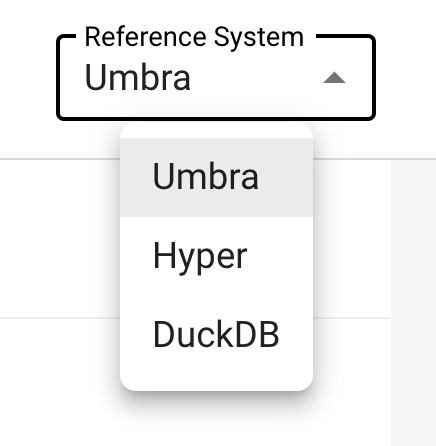
\includegraphics[width=0.3\linewidth]{figures/select-baseline-system.png}
  \caption{A drop-down menu that allows to select a baseline system.}
  \label{fig:select-baseline-system}
\end{figure}


This functionality proves useful for assessing how the performance of the chosen baseline system compares to others, aiding in the identification of strengths, weaknesses, and potential optimization areas. It forms a foundational step in the detailed analysis provided by the Benchy Viewer. Several visualisations in the application utilize the baseline system, including the table view and scatter plot for inspecting the slowdown and speedup metric, and the bar chart showcasing the performance delta for each query from the perspective of the baseline system. All these visualisations depend on a baseline system, making this functionality crucial for a comprehensive performance analysis.

In the context of providing a clear and comparative understanding of how different systems perform relative to a chosen baseline, the metrics maximum slowdown and maximum speedup become crucial. They offer a comprehensive view of the range of performance variations. Maximum slowdown indicates the worst-case scenario of reduced performance, while maximum speedup highlights the most significant improvement achieved.

\textbf{Slowdown} indicates how much slower a specific system is compared to the baseline system. It is calculated as the ratio of the time taken by the system under consideration to the time taken by the baseline system. A slowdown value greater than 1 implies that the system is slower than the baseline. For example, a slowdown of 1.5 means the system is 1.5 times slower than the baseline.\\
Identifying slowdowns is crucial for pinpointing areas of inefficiency or performance bottlenecks in a system. It helps in understanding where improvements are needed.

\textbf{Speedup}, on the other hand, quantifies how much faster a specific system is compared to the baseline system. It is calculated similarly to slowdown but in the reverse manner. A speedup value greater than 1 implies that the system is faster than the baseline. For example, a speedup of 2 means the system is twice as fast as the baseline.\\
Knowing the speedup is essential to highlight improvements. It indicates the effectiveness of optimizations or enhancements made to the system compared to the baseline.

The Benchy Viewer employs tables to showcase the maximum slowdown and maximum speedup, visualised in Figure~\ref{fig:slowdown-speedup-chart}, where the maximum slowdown is displayed on the left side and the maximum speedup on the right side using Umbra as the baseline system. The use of cell colours in the table serves as an effective visual indicator of performance outliers. Intensity in colour corresponds to the extent of the outlier, offering a rapid understanding of the range and distribution between these extreme values. This colour-coded representation aids users in identifying and assessing the significance of performance variations across different systems.

\begin{figure}[h]
  \centering
  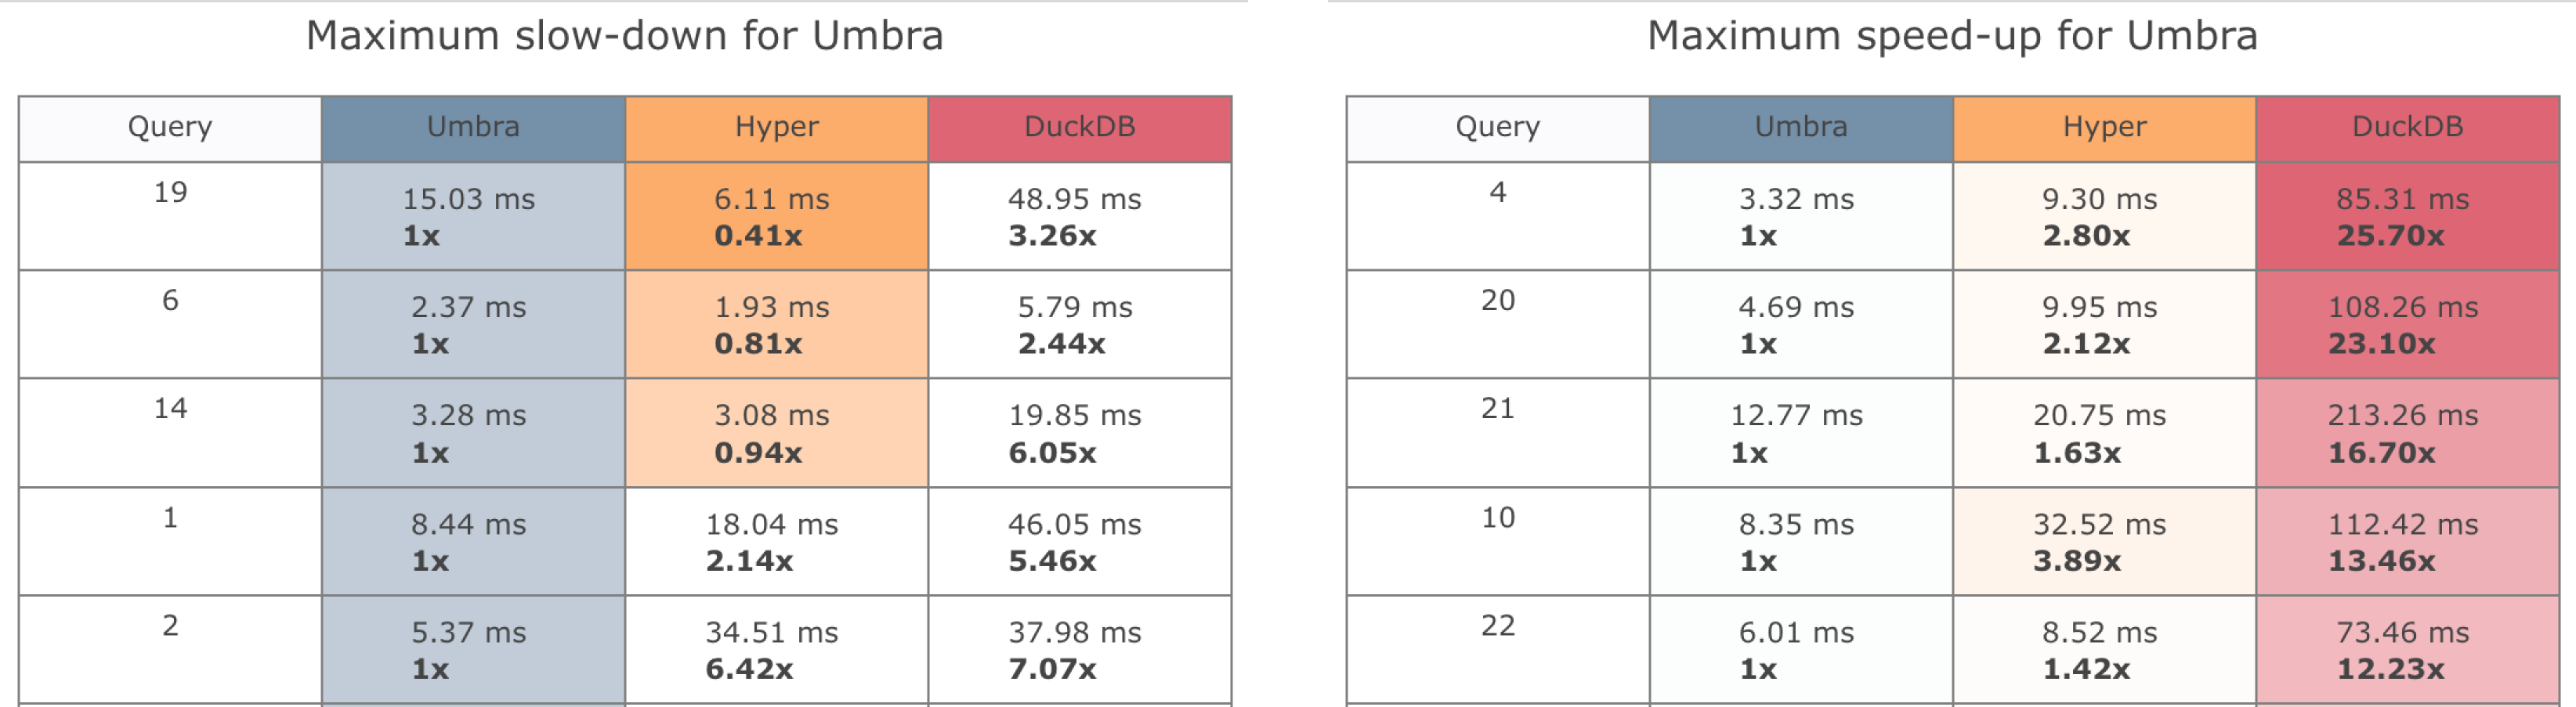
\includegraphics[width=1\linewidth]{figures/bsp-table-speedup-slowdown.png}
  \caption{Tables showcase the maximum slowdown and the maximum speedup using colour intensity to indicate performance outliers.}
  \label{fig:slowdown-speedup-chart}
\end{figure}

The tables are organized based on the resulting ratio.\\
In the maximum slowdown tables, the arrangement is ascending, placing the slowest queries of the baseline system compared to the faster alternative system at the top.\\
Conversely, in maximum speedup tables, the sorting is descending, presenting the fastest queries of the baseline system compared to the alternative system at the forefront. This sorting strategy provides a logical structure to quickly identify and compare performance differences in either scenario.

The scatter plot is another effective choice for visualising speedup and slowdown. These plots are particularly beneficial for trend analysis, offering a detailed view of each query individually. Users can identify trends, clusters, or outliers in the data, providing insights that might be less apparent in a table.

In the Benchy Viewer a baseline is displayed, as illustrated in Figure~\ref{fig:scatter} positioned at Y = 1 and coloured in blue. This positioning allows users to observe the relative performance of each query compared to the baseline system.

\begin{figure}[h]
  \centering
  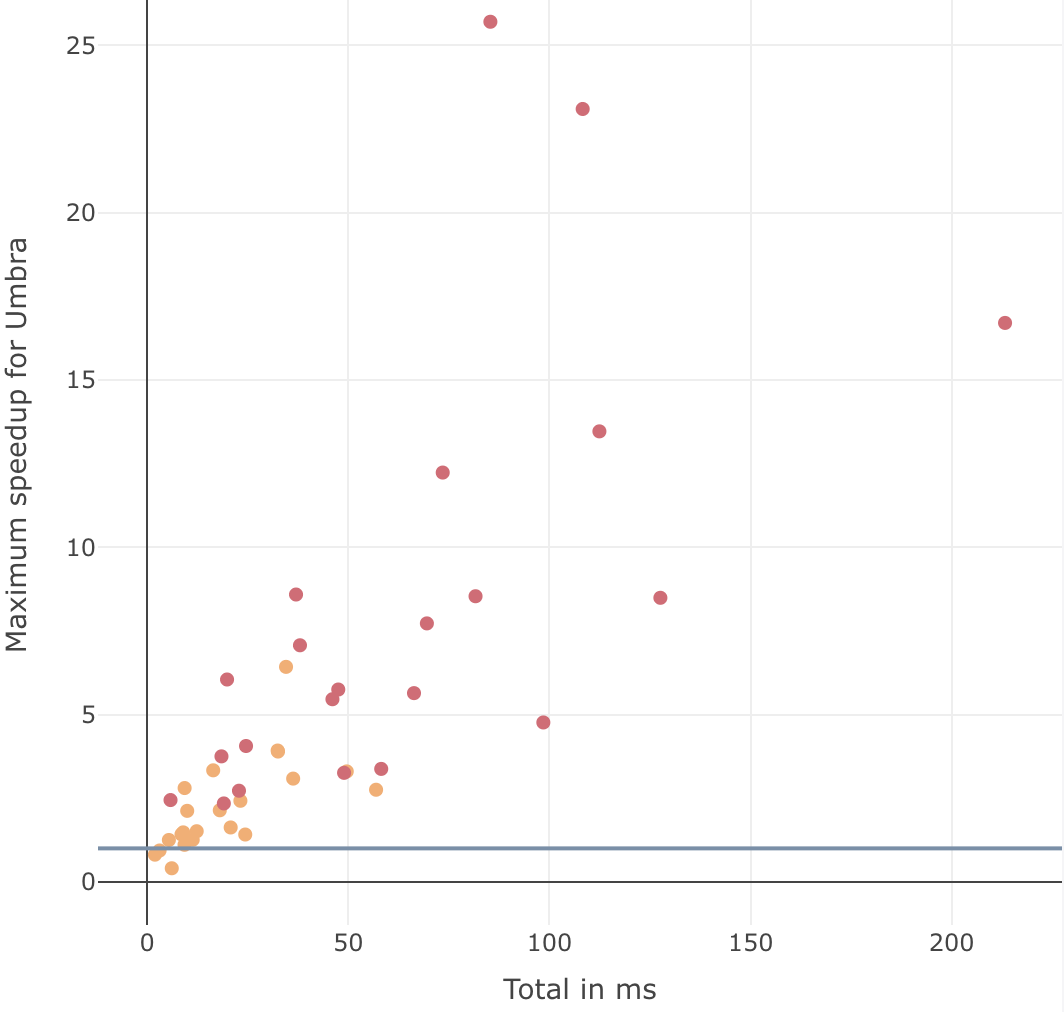
\includegraphics[width=0.7\linewidth]{figures/bsp-scatter.png}
  \caption{Scatter Plot visualises the speedup.}
  \label{fig:scatter}
\end{figure}

In this example, the scatter plot represents the maximum speedup for the selected baseline system on the Y-axis, while the total time in milliseconds is represented on the X-axis. This visualises the relationship between the total time taken by each query and its corresponding speedup compared to the baseline system.\\
Hovering above these query data points reveals the ratio of the corresponding speedup and the query identifier. We will explore the hover feature further in \ref{sec:hover-feature}.\\
Queries from the competing system are marked in orange, and most of them are slower, with three queries below the baseline, indicating that these particular queries are faster.\\
This observation prompts further investigation into the queries below the baseline, offering an opportunity to identify potential performance bottlenecks from the perspective of the baseline system. This nuanced understanding, facilitated by the visual representation of the scatter plot, guides users in pinpointing specific queries that deviate from the expected performance trend, aiding in targeted optimizations and analysis.

In the Benchy Viewer, another visualisation occurs, highlighting the performance disparities between a chosen baseline system and its competitors. It takes the form of a bar chart that illustrates the performance gap for each query, providing a perspective of the baseline system compared to the best-performing query of other competing systems.

The performance delta chart in the Benchy Viewer not only displays the performance gap for each query from the perspective of the baseline system but also indicates the best competing system for each query by using corresponding system colours, as depicted in Figure~\ref{fig:performance-gap}. The Y-axis shows the performance gap percentage of the competing queries, while the X-axis represents the identifying query number. Hovering over bars reveals the exact performance delta.

\begin{figure}[h]
  \centering
  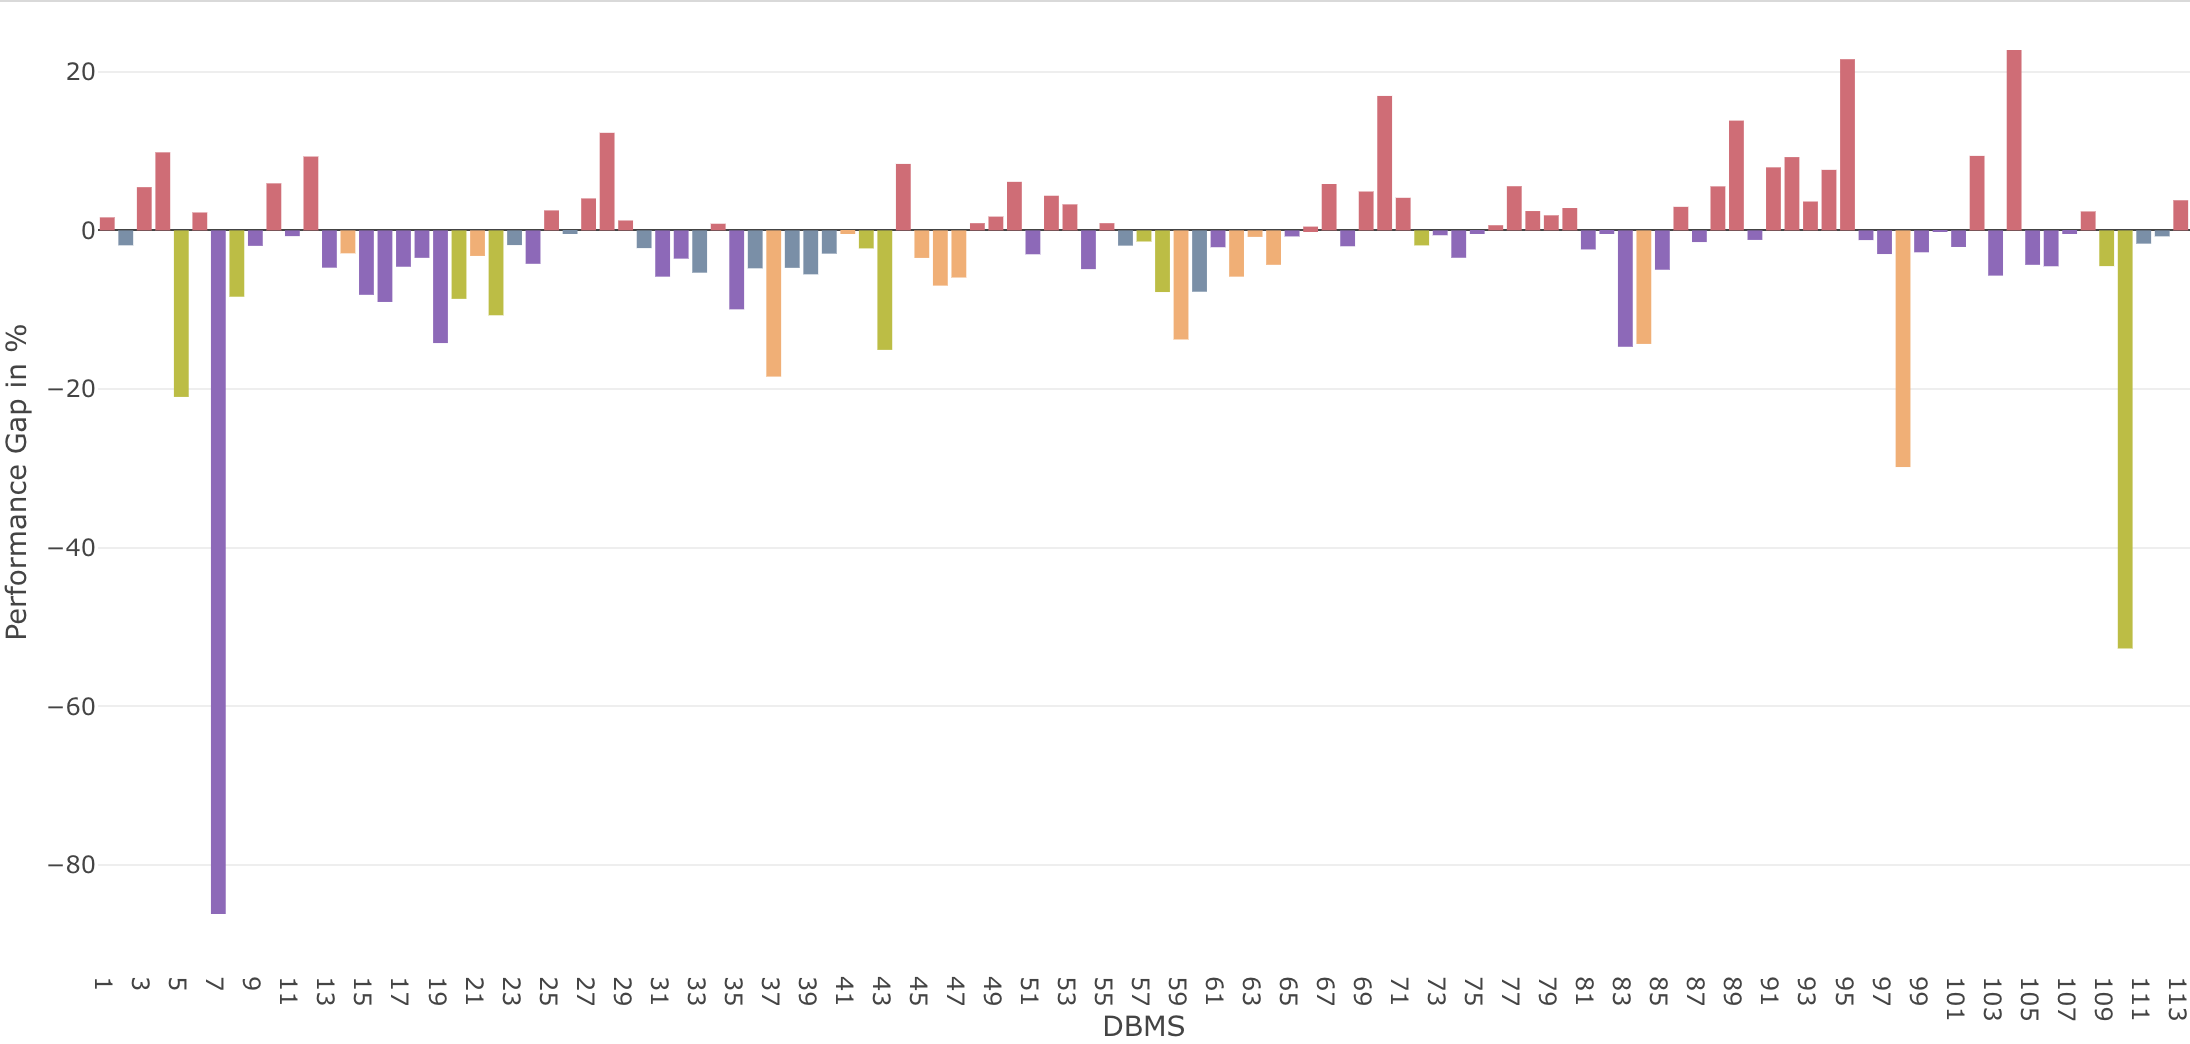
\includegraphics[width=1\linewidth]{figures/bsp-query-gaps.png}
  \caption{Bar chart visualises the performance gap for every query of the baseline system compared to best corresponding query of the competing systems.}
  \label{fig:performance-gap}
\end{figure}

In this example, the red-marked database system is selected as the baseline system. Queries with faster performance by the baseline system are displayed above the baseline, indicating a positive performance delta. In contrast, queries with stronger performance by competing systems are shown below the baseline, indicating a negative performance delta for the baseline system. Additionally, the bar of each query is marked with the colour of the corresponding best-performing database system.\\
The performance gap for the majority of cases in this example stays within a range between -20\% and 20\%. However, some outliers are notably significant. For instance, the seventh query has a performance gap of -86\%. A deeper analysis of this query may be sensible to potentially identify performance bottlenecks from the perspective of the baseline system.

This query performance gap visualisation is instrumental in quickly discerning how each query of the baseline system stacks up against the top-performing queries of other systems. The chart's simplicity ensures easy comprehension, enabling users to promptly assess the relative performance of different queries.




\subsubsection{Hover Feature}\label{sec:hover-feature}

\begin{figure}[h]
  \centering
  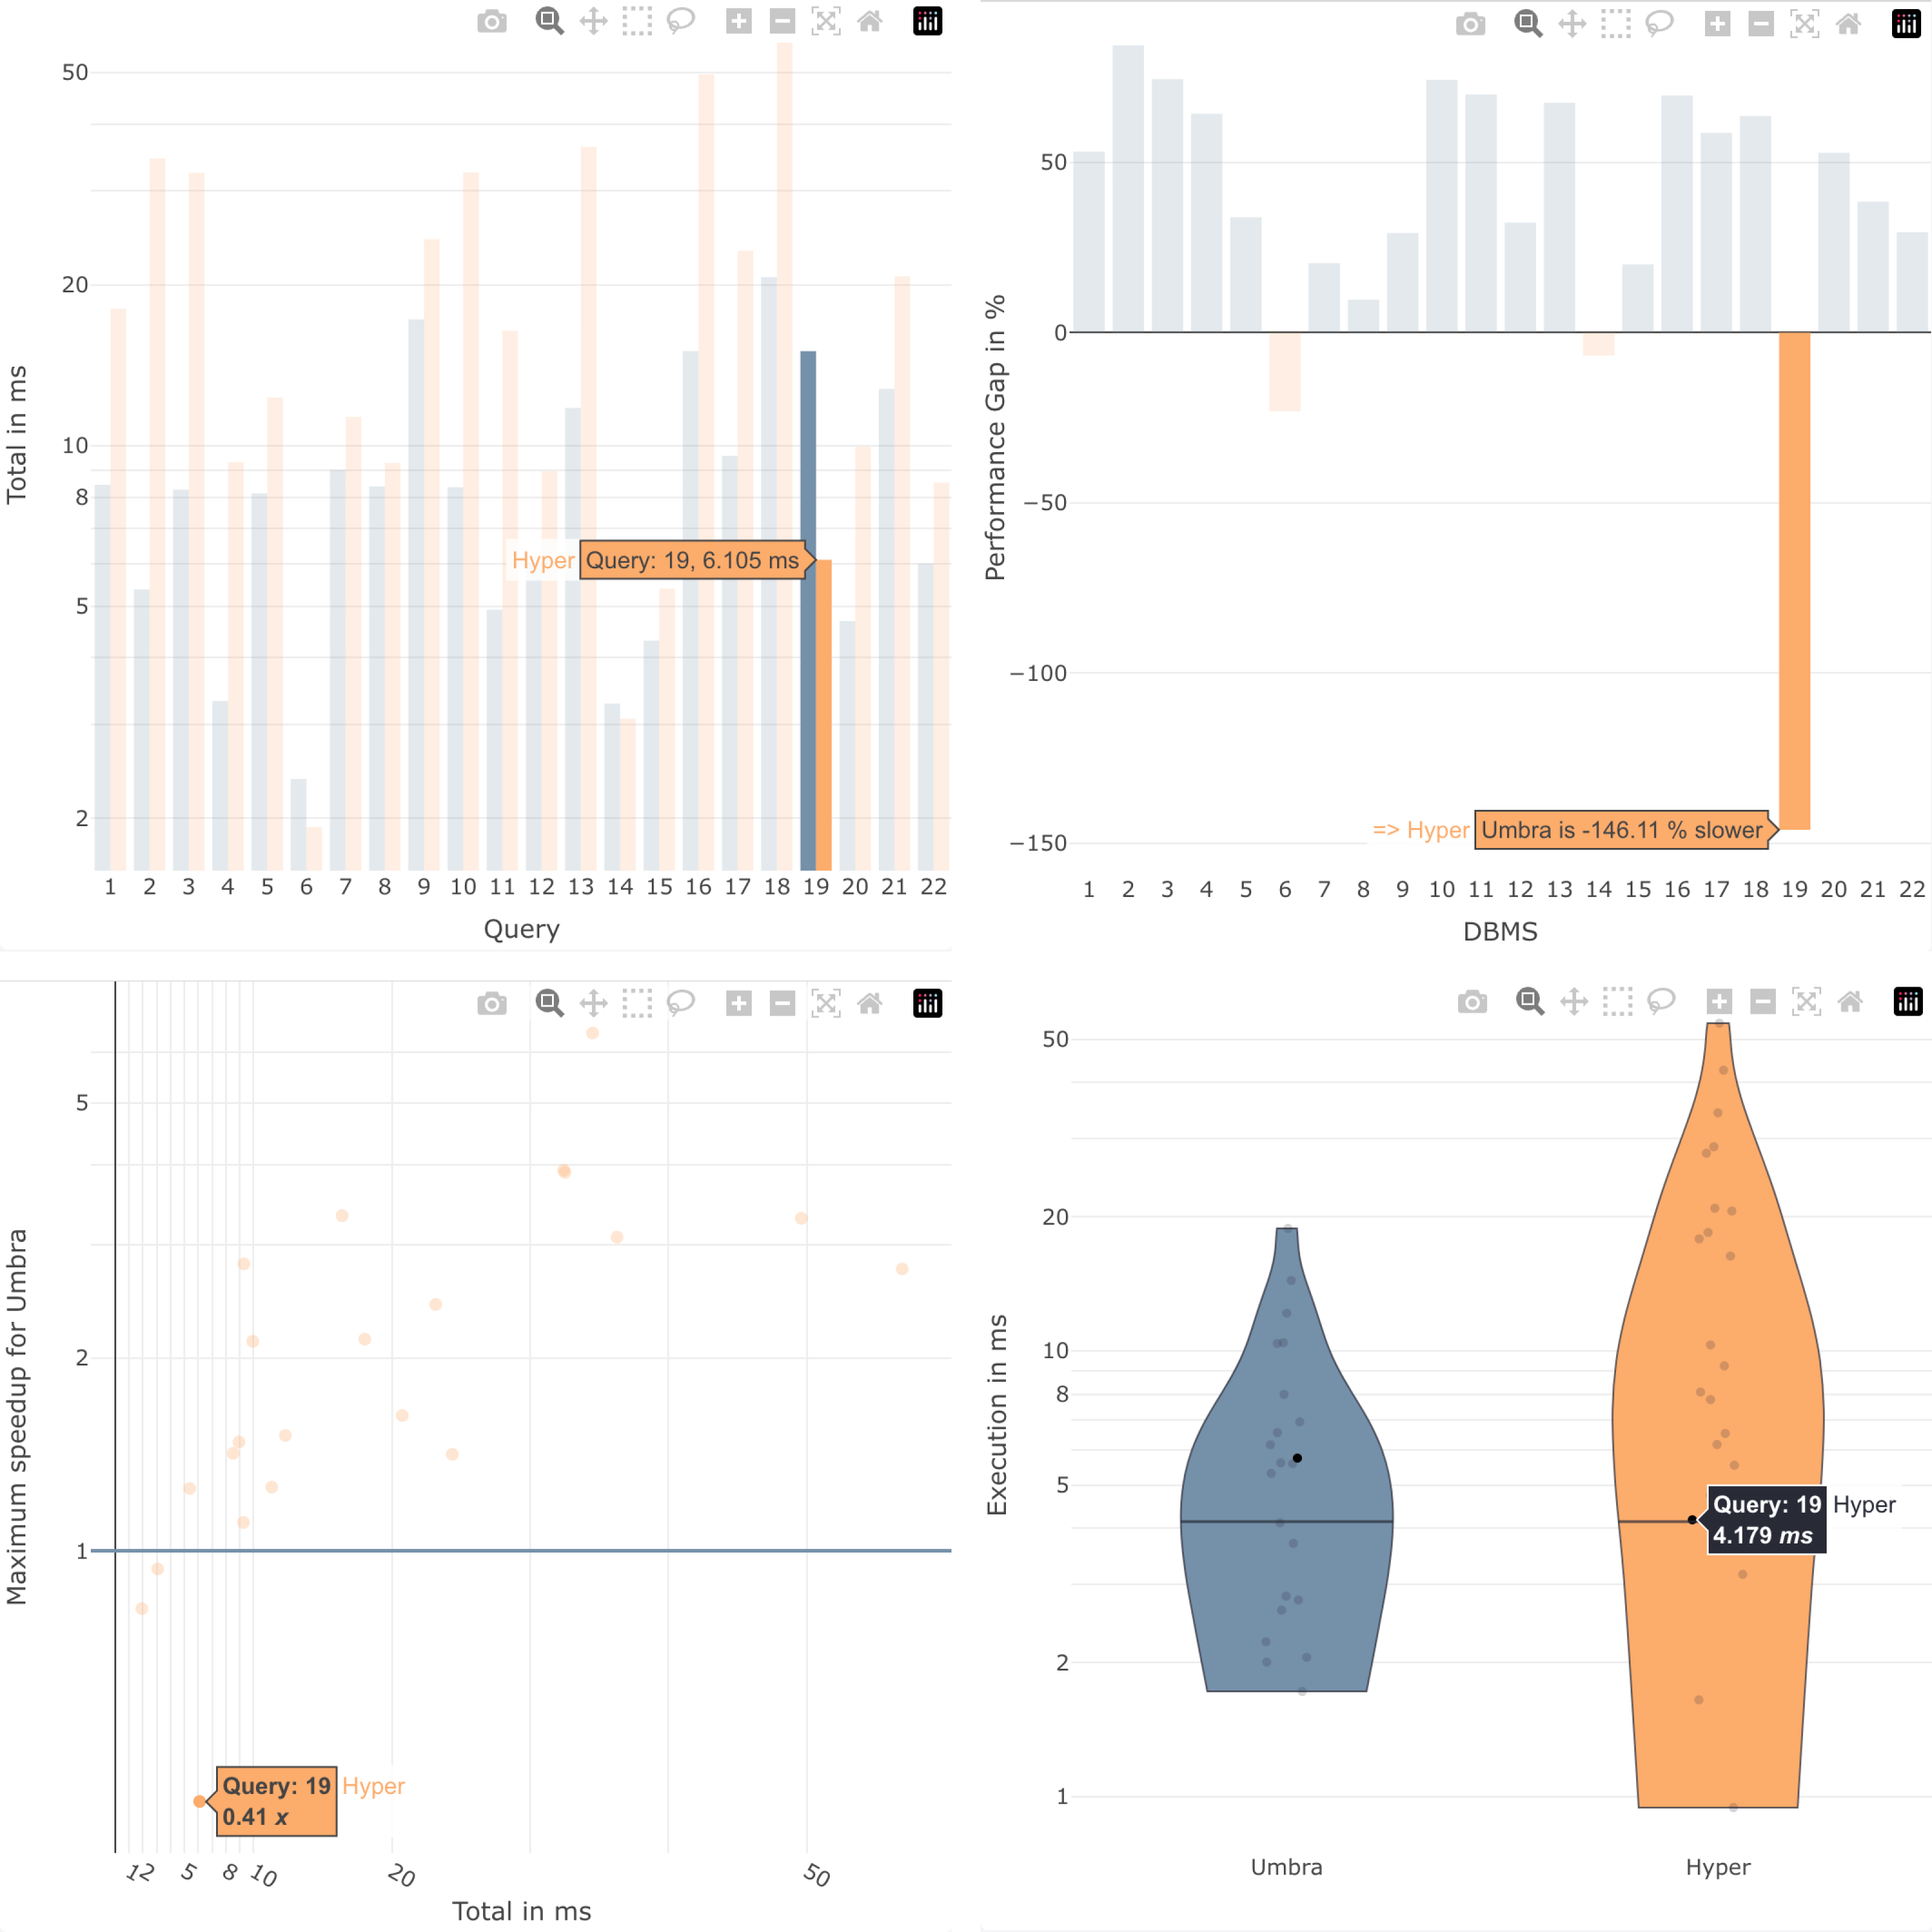
\includegraphics[width=0.6\linewidth]{figures/hover-group.png}
  \caption{Hovering over a query automatically highlights in a global context the same query in all visualisations which are showcasing single queries. These visualisations include violin plots, scatter plots, and bar charts when one bar represents a single query.}
  \label{fig:hover-group}
\end{figure}

Hovering over data points in a chart is an indispensable feature, commonly employed to extract more detailed information about a specific data point. In the context of analysing query performances and identifying noteworthy queries within visualisations, the ability to scrutinize a particular query from multiple perspectives becomes crucial.


 In the Benchy Viewer, we've elevated this feature, which is illustrated in Figure~\ref{fig:hover-group}, to a global hover capability within the application.\\
 This means that when a user hovers over a specific query, not only is that query highlighted within the current chart, but the same queries within all other visualizations are also highlighted simultaneously.This synchronization spans various visualizations, including violin plots, scatter plots, and bar charts which represent distinct queries.



\subsubsection{Data Viewer}

In addition to visualisations, the Benchy Viewer features a data table for in-depth inspection of benchmark data. This table presents the imported user data, as exemplified in the excerpt of the data viewer in Figure~\ref{fig:data-viewer}.

\begin{figure}[h]
  \centering
  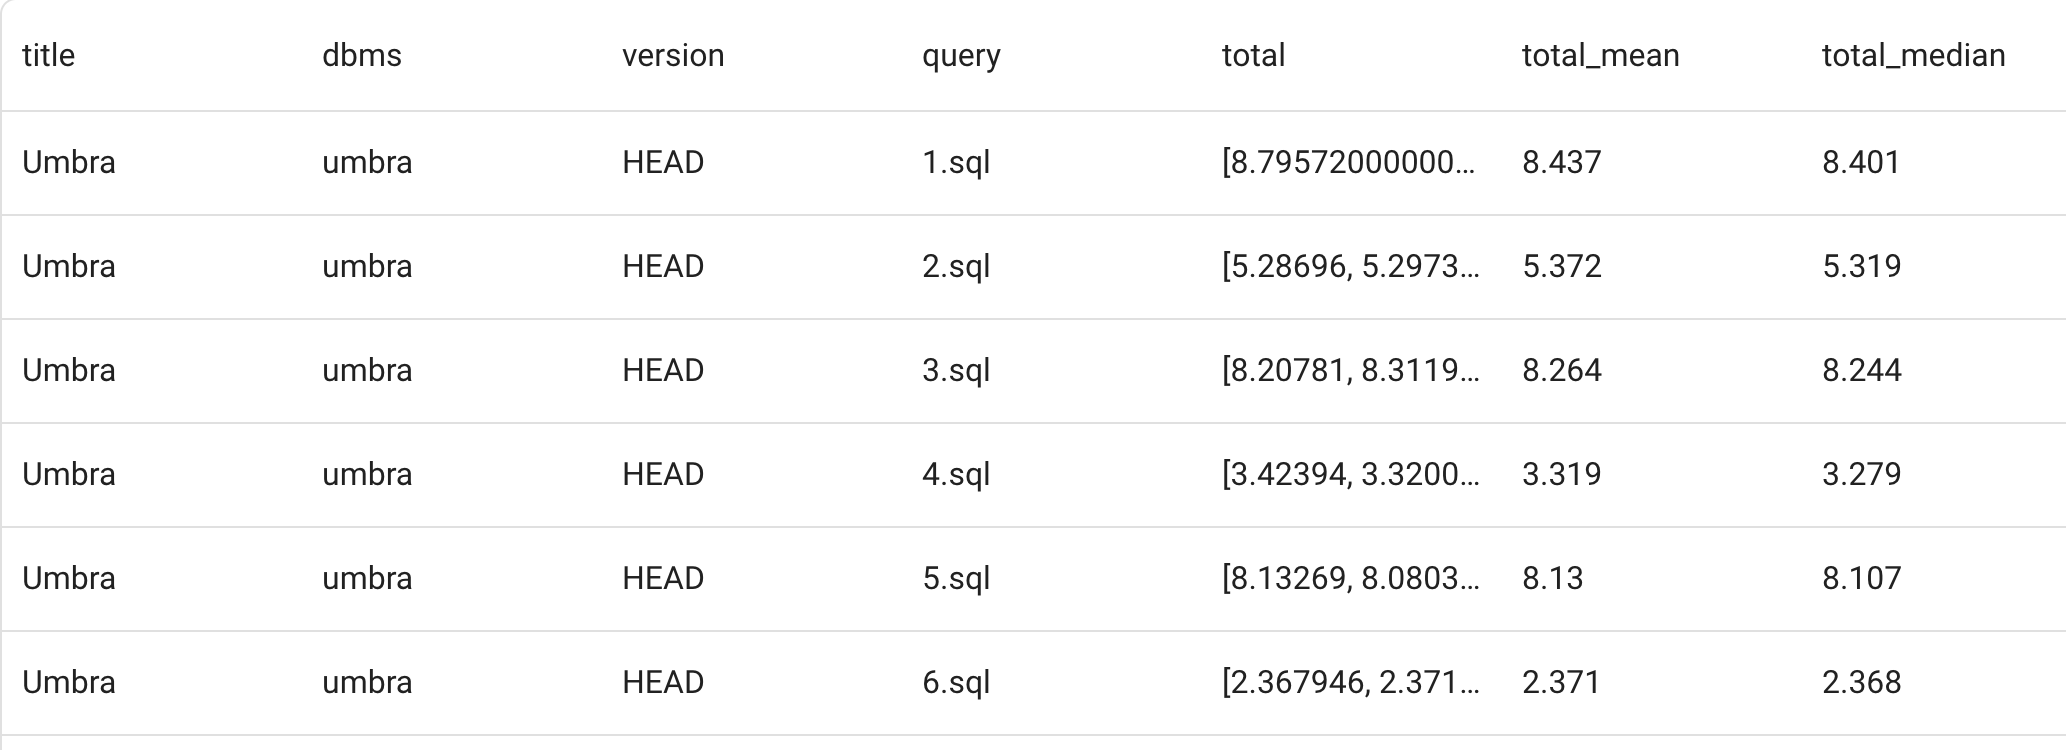
\includegraphics[width=0.9\linewidth]{figures/data-viewer.png}
  \caption{.}
  \label{fig:data-viewer}
\end{figure}

This view displays the complete data, which is described deeply in section \ref{sec:input-file-structure}.\\
The header contains all properties and metrics of a data row. The data rows below the header represent the data of a query, containing the reference to the database system and the complete benchmark data of this query.\\
The user can scroll vertically and horizontally given the amount of the data rows and the metrics. The header provides some options in a drop-down menu to work with the data sheet, as shown in Figure~\ref{fig:data-viewer-options}. The first option is to sort the table by a chosen data column containing numerical data. The user has the possibility to do this ascending or descending and also reset the sorting. This is useful when the user wants to sort specific data, e.g. the total time in ms.


This view showcases the benchmark data, elaborately described in Section \ref{sec:input-file-structure}. The header encompasses all properties and metrics of a data row. Data rows below the header represent the data of a query, including the reference to the database system and the complete benchmark data for that query.\\
Vertical and horizontal scrolling are enabled to navigate through the extensive data rows and metrics, as the volume of information exceeds the screen's capacity.

\begin{figure}[h]
  \centering
  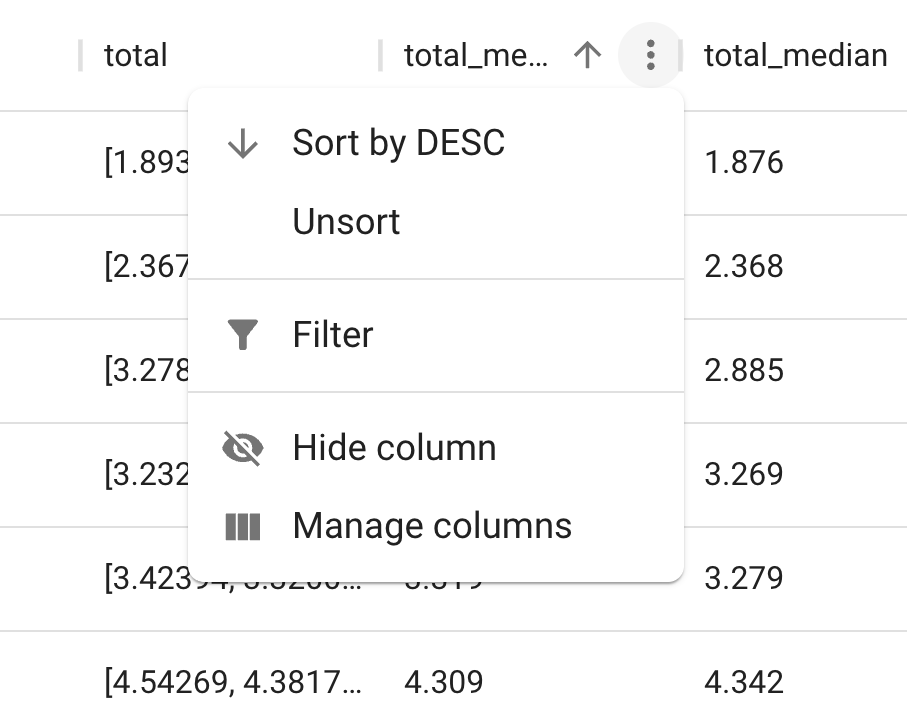
\includegraphics[width=0.4\linewidth]{figures/data-viewer-header-options.png}
  \caption{.}
  \label{fig:data-viewer-options}
\end{figure}

The header offers various options in a drop-down menu to interact with the data sheet, as depicted in Figure~\ref{fig:data-viewer-options}.

% Sorting
The first option enables sorting the table based on a selected data column with numerical values. Users can choose between ascending or descending order, and there's an option to reset the sorting. This functionality is particularly useful when organizing specific data, for instance, sorting the table based on total time in milliseconds.

\begin{figure}[h]
  \centering
  \begin{subfigure}[b]{0.4\linewidth}
      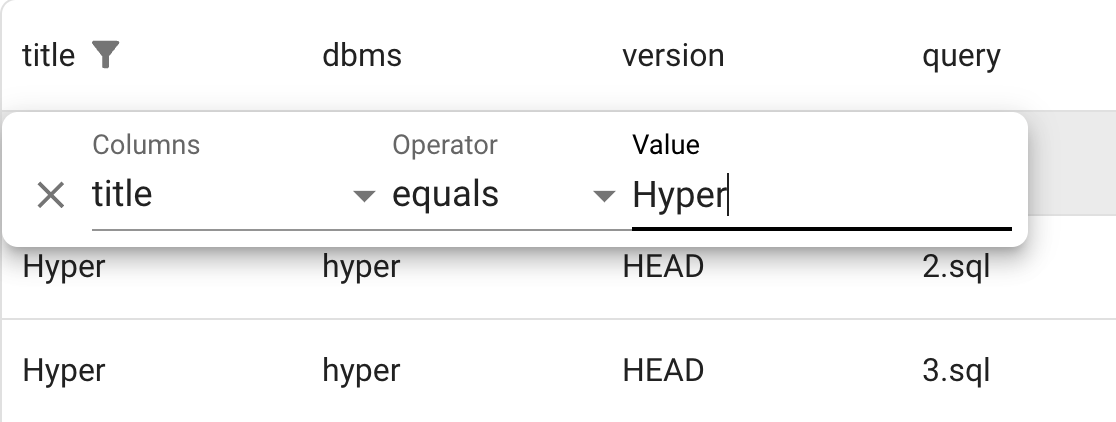
\includegraphics[width=\linewidth]{figures/data-viewer-filter.png}
      \caption{Caption for Figure 1.}
      \label{fig:data-viewer-filter}
  \end{subfigure}
  \hspace{1cm} % Adjust the horizontal space between the figures
  \begin{subfigure}[b]{0.4\linewidth}
      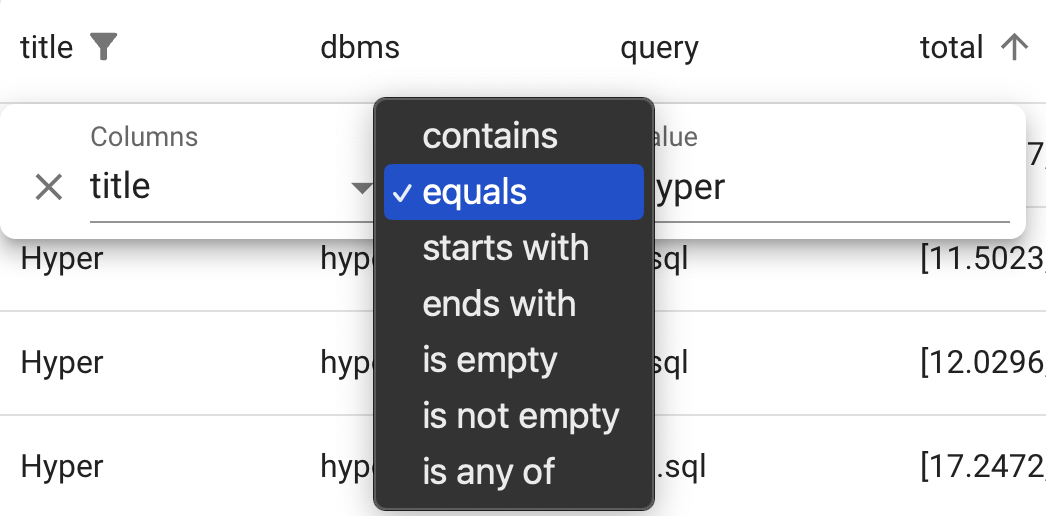
\includegraphics[width=\linewidth]{figures/data-viewer-filter-operator.png}
      \caption{Caption for Figure 2.}
      \label{fig:data-viewer-filter-operator}
  \end{subfigure}
  \caption{Overall caption for both figures.}
  \label{fig:combined-figures}
\end{figure}

% Filter
The filter option, as shown in Figure~\ref{fig:data-viewer-filter}, provides a tool for refining the displayed data in the table. Users can easily narrow down their focus by selecting a specific column, an operator, and a value. This allows for targeted exploration of the data, such as isolating rows related to a particular database management system, as demonstrated in Figure~\ref{fig:data-viewer-filter-operator}. This filtering capability enhances the user's ability to extract meaningful insights from the benchmark data.


% Manage Columns

\begin{figure}[h]
  \centering
  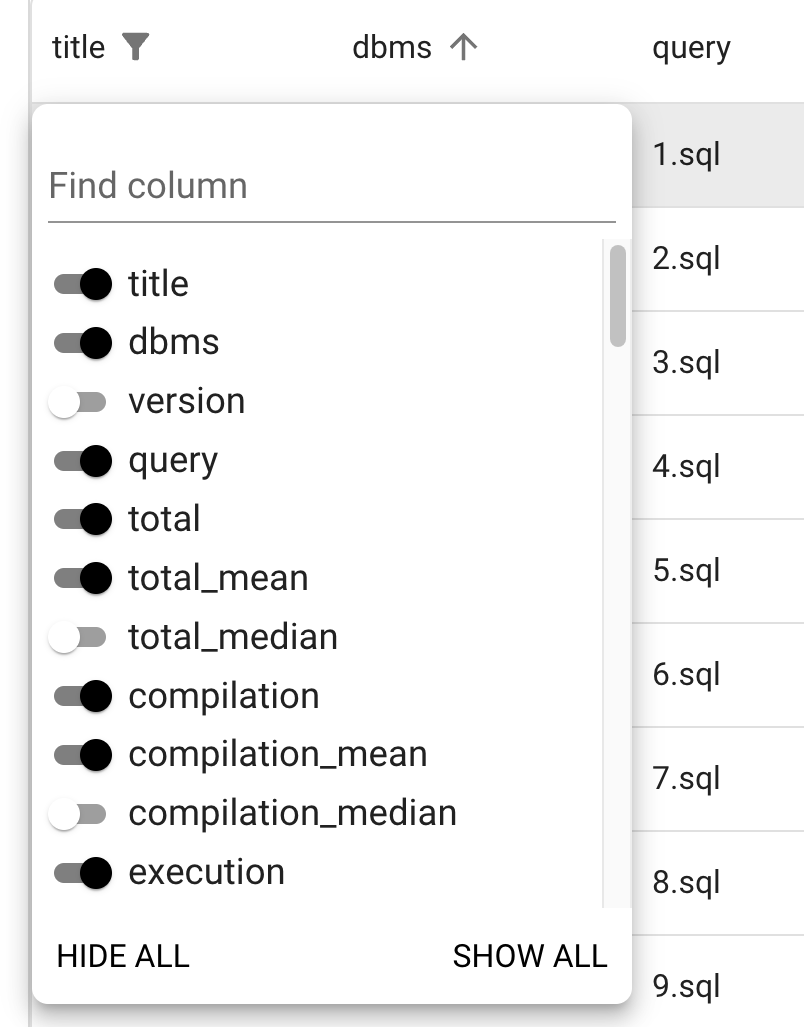
\includegraphics[width=0.35\linewidth]{figures/data-viewer-manage-columns.png}
  \caption{.}
  \label{fig:data-viewer-manage-columns}
\end{figure}

When dealing with extensive datasets, the Benchy Viewer ensures flexibility and ease of use by allowing users to tailor their view. Through the 'Manage columns' feature, accessed via the drop-down menu, users can not only hide columns but also gain a holistic overview of active columns. 

Figure~\ref{fig:data-viewer-manage-columns} showcases this functionality, providing users with the ability to effortlessly activate or deactivate columns, conduct quick searches, and streamline their view by hiding or showing all columns at once. This empowers users to focus on the specific data points relevant to their analysis, enhancing the efficiency of the benchmark data exploration process.




\subsection{Deeper Inspection and Comparison of selected Queries}
Query Plan
DBs aktivieren/ deaktivieren
\subsection{Flexible Interface Hub}
\subsubsection{Drag and Drop}
DnD Sektionen und Dnd Charts
\subsubsection{Chart Configurations}
- Metrics auswählen
- tabele und scatter: speed-up/ slow-down
- Scale: Linear/ Log/ Throuput
- Violin: scatter und boxplot
\subsection{Saving and Sharing the Application State}


\section{Design}
\subsection{User Interface}
\subsection{Page Structure and Navigation}
\subsubsection{}

\section{Data Structure}
\subsection{Overall Project Structure}
\subsection{Input File and Benchmark Data}


\subsubsection{Import of Performance Data}

The first step, working with the Benchy Viewer is to import a file containing the performance data which should be visualised. The file needs to follow the format introduced in Section \ref{sec:input-file-structure}. Figure~\ref{fig:input-process-flow} summarizes the import of the input file in a process diagram.

\begin{figure}[h]
  \centering
  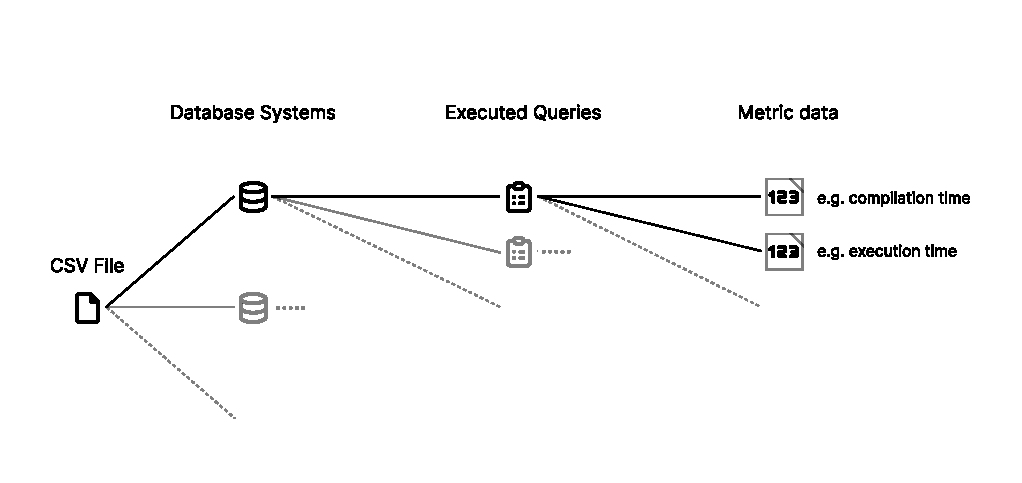
\includegraphics[width=1\linewidth]{figures/csv-structure.pdf}
  \caption{Import process of input data}
  \label{fig:input-process-flow}
\end{figure}

Chart beschreiben.


\subsection{Plot Options}
\subsection{Visualisation Arrangement Data Structure}
\subsection{Query Plan}
\subsubsection{Visualisation Parameters}
\subsubsection{Query Plan Data Structure}

\section{Integration of Plotly-React for Data Visualisation}
\subsection{Types of Plots and Charts}
\subsection{Hover Feature}
\subsection{Selected Query Feature}

\section{Integration of semantic-diff-tool}
\subsection{Business Logic}
\subsection{Settings}
\subsection{UI}